\section{Path Style}

\subsection{样式概述}

在 path 中添加修饰是十分自由的,在路径的任意地点添加的全局修饰都将起到相同的效果,同一段路径也允许有多个修饰,以下语句的效果相同。

\begin{lstlisting}[style = latex-side]
    \path [draw,fill] (0,0) circle (1cm);
    \path [draw] [fill] (0,0) circle (1cm);
    \path [fill] (0,0) circle (1cm) [draw];
    \draw [fill] (0,0) circle (1cm);
    \fill (0,0) [draw] circle (1cm);
    \filldraw (0,0) circle (1cm);
\end{lstlisting}

下面指令都是基于 \textbackslash path 指令衍生出来的常用指令:
\begin{itemize}
    \item \textbackslash draw  
    
    等效于 \textbackslash path[draw];绘制边线。
    \item \textbackslash fill 
    
    等效于 \textbackslash path[fill];填充颜色。
    \item \textbackslash filldraw
    
    等效于 \textbackslash path[fill,draw];绘制边线并填充颜色。
    \item \textbackslash pattern  
    
    等效于 \textbackslash path[pattern];填充图案。
    \item \textbackslash shade  
    
    等效于 \textbackslash path[shade];产生投影。
    \item \textbackslash shadedraw  
    
    等效于 \textbackslash path[shadedraw];绘制边线与投影。
    \item \textbackslash clip  
    
    等效于 \textbackslash path[clip];切片?
    \item \textbackslash useasboundingbox  
    
    等效于 \textbackslash path[useasboundingbox];绘制边框。
\end{itemize}


路径具有多种修饰,且部分修饰的值可能会重复,例如 color,有 fill = <color>,draw = <color> 等,如果不指定修饰名(键)则默认全部相关修饰均采用。

\begin{figure}[H]
    \centering
    \begin{minipage}{0.35\linewidth}
        \centering
        
\begin{tikzpicture}[scale = 1]
            \path[yshift = 0cm, fill = red!20] (0,0) circle (1ex);
            \path[yshift = 2em, draw = red!20] (0,0) circle (1ex);
            \path[yshift = 4em, red!20,fill,draw] (0,0) circle (1ex);
        \end{tikzpicture}
    \end{minipage}
    \begin{minipage}{0.55\linewidth}
        \begin{lstlisting}[style = latex-side]
    
\begin{tikzpicture}[scale = 1]
        \path[yshift = 0cm, fill = red!20] (0,0) circle (1ex);
        \path[yshift = 2em, draw = red!20] (0,0) circle (1ex);
        \path[yshift = 4em, red!20,fill,draw] (0,0) circle (1ex);
    \end{tikzpicture}
        \end{lstlisting}
    \end{minipage}
    \caption{Path Style:color}
\end{figure}

\subsection{线条样式}
\subsubsection{线条粗细}

\begin{itemize}
    \item line width = <dimension> \hfill (默认:0.4pt)
    
    控制线条粗细,该键可以省略。

    \begin{figure}[H]
        \centering
        \begin{minipage}{0.35\linewidth}
            \centering
            
\begin{tikzpicture}[scale = 1]
                \draw[line width = 5pt] (0,0) -- (3,0);
            \end{tikzpicture}
        \end{minipage}
        \begin{minipage}{0.55\linewidth}
            \begin{lstlisting}[style = latex-side]
    \draw[line width = 5pt] (0,0) -- (3,0);
            \end{lstlisting}
        \end{minipage}
        \caption{Path Style:line width}
    \end{figure}

    TikZ 为我们预设了几种常用的粗细,它们的值如下:

    \begin{table}[H]
        \centering
        \caption{line width:预设值}
        \label{table:line width:预设值}
        \setlength{\tabcolsep}{5mm}
        \begin{tabular}{cc|cc|cc}
            \toprule
            \textbf{名称} & \textbf{粗细} & \textbf{名称} & \textbf{粗细} & \textbf{名称} & \textbf{粗细} \\
            \midrule
            ultra thin  & 0.1pt  & very thin & 0.2pt & thin & 0.4pt \\
            semithick   & 0.6pt  & thick     & 0.8pt & very thick & 1.2pt \\
            ultra thick   & 1.6pt  &&&& \\
            \bottomrule
        \end{tabular}
    \end{table}

    \begin{figure}[H]
        \centering
        \begin{minipage}{0.35\linewidth}
            \centering
            
\begin{tikzpicture}[scale = 1]
                \draw [yshift = 0,    ultra thin]   (0,0) -- (3,0);
                \draw [yshift = -1em, very thin]    (0,0) -- (3,0);
                \draw [yshift = -2em, thin]         (0,0) -- (3,0);
                \draw [yshift = -3em, semithick]    (0,0) -- (3,0);
                \draw [yshift = -4em, thick]        (0,0) -- (3,0);
                \draw [yshift = -5em, very thick]   (0,0) -- (3,0);
                \draw [yshift = -6em, ultra thick]  (0,0) -- (3,0);
            \end{tikzpicture}
        \end{minipage}
        \begin{minipage}{0.55\linewidth}
            \begin{lstlisting}[style = latex-side]
    \draw [yshift = 0,    ultra thin]   (0,0) -- (3,0);     % 0.1pt
    \draw [yshift = -1em, very thin]    (0,0) -- (3,0);     % 0.2pt
    \draw [yshift = -2em, thin]         (0,0) -- (3,0);     % 0.4pt
    \draw [yshift = -3em, semithick]    (0,0) -- (3,0);     % 0.6pt
    \draw [yshift = -4em, thick]        (0,0) -- (3,0);     % 0.8pt
    \draw [yshift = -5em, very thick]   (0,0) -- (3,0);     % 1.2pt
    \draw [yshift = -6em, ultra thick]  (0,0) -- (3,0);     % 1.6pt
            \end{lstlisting}
        \end{minipage}
        \caption{Path Style:线条粗细关键字}
    \end{figure}

\end{itemize}

\subsubsection{描边样式}
\begin{itemize}
    \item line cap = <type> \hfill (默认:butt)
    
    用于指明线条端点样式,有 round,rect,butt 三种样式:

    \begin{figure}[H]
        \centering
        \begin{minipage}{0.35\linewidth}
            \centering
            
\begin{tikzpicture}[scale = 1]
                \begin{scope}[line width=10pt]
                    \draw[line cap=round] (0,1 ) -- +(3,0);
                    \draw[line cap=butt] (0,.5) -- +(3,0);
                    \draw[line cap=rect] (0,0 ) -- +(3,0);
                \end{scope}
                \draw[white,line width=1pt]
                    (0,0 ) -- +(3,0) (0,.5) -- +(3,0) (0,1 ) -- +(3,0);
            \end{tikzpicture}
        \end{minipage}
        \begin{minipage}{0.55\linewidth}
            \begin{lstlisting}[style = latex-side]
    
\begin{tikzpicture}[scale = 1]
        \begin{scope}[line width=10pt]
            \draw[line cap=round] (0,1 ) -- +(3,0);
            \draw[line cap=butt] (0,.5) -- +(3,0);
            \draw[line cap=rect] (0,0 ) -- +(3,0);
        \end{scope}
        \draw[white,line width=1pt]
            (0,0 ) -- +(3,0) (0,.5) -- +(3,0) (0,1 ) -- +(3,0);
    \end{tikzpicture}
            \end{lstlisting}
        \end{minipage}
        \caption{Path Style:line cap}
    \end{figure}

    \item line join = <type> \hfill (默认:miter)
    
    用于指定线条拐角处的样式,有 round,bevel,miter 三种。

    \begin{figure}[H]
        \centering
        \begin{minipage}{0.35\linewidth}
            \centering
            \begin{tikzpicture}[scale = 1]
                \begin{tikzpicture}[line width=10pt]
                    \draw[line join=round] (0,0) -- ++(.5,1) -- ++(.5,-1);
                    \draw[line join=bevel] (1.25,0) -- ++(.5,1) -- ++(.5,-1);
                    \draw[line join=miter] (2.5,0) -- ++(.5,1) -- ++(.5,-1);
                    \useasboundingbox (0,1.5); % enlarge bounding box
                \end{tikzpicture}
            \end{tikzpicture}
        \end{minipage}
        \begin{minipage}{0.55\linewidth}
            \begin{lstlisting}[style = latex-side]
    
\begin{tikzpicture}[line width=10pt]
        \draw[line join=round] (0,0) -- ++(.5,1) -- ++(.5,-1);
        \draw[line join=bevel] (1.25,0) -- ++(.5,1) -- ++(.5,-1);
        \draw[line join=miter] (2.5,0) -- ++(.5,1) -- ++(.5,-1);
        \useasboundingbox (0,1.5); % enlarge bounding box
    \end{tikzpicture}
            \end{lstlisting}
        \end{minipage}
        \caption{Path Style:line join}
    \end{figure}

    \item miter limit = <factor>  \hfill (默认:10)
    
    当夹角过小时,拐角处往往会显得过尖,用 miter limit 可以限制这一情况。

    \begin{figure}[H]
        \centering
        \begin{minipage}{0.7\linewidth}
            \centering
            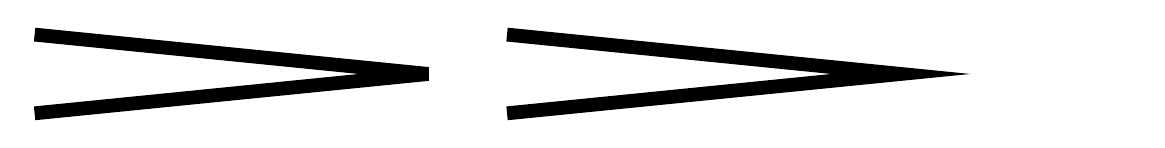
\begin{tikzpicture}[line width=5pt]
                \draw (0,0) -- ++(5,.5) -- ++(-5,.5);
                \draw[miter limit=25] (6,0) -- ++(5,.5) -- ++(-5,.5);
                \useasboundingbox (14,0); % make bounding box bigger
            \end{tikzpicture}
        \end{minipage}
        \begin{minipage}{0.7\linewidth}
            \begin{lstlisting}[style = latex-side]
    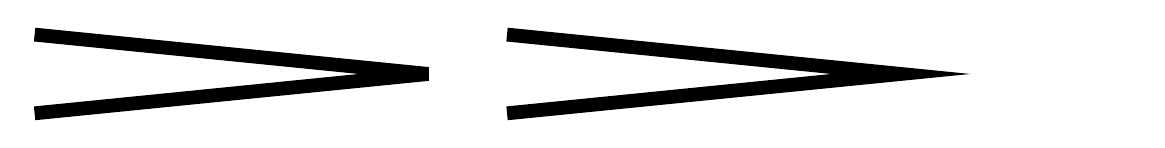
\begin{tikzpicture}[line width=5pt]
        \draw (0,0) -- ++(5,.5) -- ++(-5,.5);
        \draw[miter limit=25] (6,0) -- ++(5,.5) -- ++(-5,.5);
        \useasboundingbox (14,0); % make bounding box bigger
    \end{tikzpicture}
            \end{lstlisting}
        \end{minipage}
        \caption{Path Style:miter limit}
    \end{figure}

\end{itemize}

\subsubsection{虚线样式}

\begin{itemize}
    \item dash pattern = <dash pattern>
    
    设置虚线样式,值中有两个关键字 on 表示绘制,off 表示空缺。

    \begin{figure}[H]
        \centering
        \begin{minipage}{0.35\linewidth}
            \centering
            \begin{tikzpicture}[dash pattern=on 2pt off 3pt on 4pt off 4pt]
                \draw (0pt,0pt) -- (3.5cm,0pt);
            \end{tikzpicture}
        \end{minipage}
        \begin{minipage}{0.55\linewidth}
            \begin{lstlisting}[style = latex-side]
    \begin{tikzpicture}[dash pattern=on 2pt off 3pt on 4pt off 4pt]
        \draw (0pt,0pt) -- (3.5cm,0pt);
    \end{tikzpicture}
            \end{lstlisting}
        \end{minipage}
        \caption{Path Style:dash pattern}
    \end{figure}

    \item dash phase = <dash phase>
    
    设置线条的起始位置。

    \begin{figure}[H]
        \centering
        \begin{minipage}{0.35\linewidth}
            \centering
            \begin{tikzpicture}[dash pattern=on 20pt off 10pt]
                \draw[dash phase=0pt] (0pt,3pt) -- (3.5cm,3pt);
                \draw[dash phase=10pt] (0pt,0pt) -- (3.5cm,0pt);
            \end{tikzpicture}
        \end{minipage}
        \begin{minipage}{0.55\linewidth}
            \begin{lstlisting}[style = latex-side]
    \begin{tikzpicture}[dash pattern=on 20pt off 10pt]
        \draw[dash phase=0pt] (0pt,3pt) -- (3.5cm,3pt);
        \draw[dash phase=10pt] (0pt,0pt) -- (3.5cm,0pt);
    \end{tikzpicture}
            \end{lstlisting}
        \end{minipage}
        \caption{Path Style:dash phase}
    \end{figure}

    \item dash = <dash pattern> phase <dash phase>
    
    可以将上面两个修饰合并为一个。

    \begin{figure}[H]
        \centering
        \begin{minipage}{0.35\linewidth}
            \centering
            \begin{tikzpicture}[scale = 1]
                \begin{tikzpicture}
                    \draw [dash=on 20pt off 10pt phase 0pt] (0pt,3pt) -- (3.5cm,3pt);
                    \draw [dash=on 20pt off 10pt phase 10pt] (0pt,0pt) -- (3.5cm,0pt);
                \end{tikzpicture}
            \end{tikzpicture}
        \end{minipage}
        \begin{minipage}{0.55\linewidth}
            \begin{lstlisting}[style = latex-side]
    \begin{tikzpicture}
        \draw [dash=on 20pt off 10pt phase 0pt] (0pt,3pt) -- (3.5cm,3pt);
        \draw [dash=on 20pt off 10pt phase 10pt] (0pt,0pt) -- (3.5cm,0pt);
    \end{tikzpicture}
            \end{lstlisting}
        \end{minipage}
        \caption{Path Style:dash}
    \end{figure}

    \item dash expand off 
    
    当路径长度不是一个 on 与 off 的整数倍时,往往会出现被截断的线段,使用该修饰可以强制使用完整的线段,将 off 增长以填充多余的区域。需要加载 decorations 包。

    \begin{figure}[H]
        \centering
        \begin{minipage}{0.35\linewidth}
            \centering
            \begin{tikzpicture}[|-|, dash pattern=on 4pt off 2pt]
                \draw [dash expand off] (0pt,30pt) -- (26pt,30pt);
                \draw [dash expand off] (0pt,20pt) -- (24pt,20pt);
                \draw [dash expand off] (0pt,10pt) -- (22pt,10pt);
                \draw [dash expand off] (0pt, 0pt) -- (20pt, 0pt);
            \end{tikzpicture}
        \end{minipage}
        \begin{minipage}{0.55\linewidth}
            \begin{lstlisting}[style = latex-side]
    \begin{tikzpicture}[|-|, dash pattern=on 4pt off 2pt]
        \draw [dash expand off] (0pt,30pt) -- (26pt,30pt);
        \draw [dash expand off] (0pt,20pt) -- (24pt,20pt);
        \draw [dash expand off] (0pt,10pt) -- (22pt,10pt);
        \draw [dash expand off] (0pt, 0pt) -- (20pt, 0pt);
    \end{tikzpicture}
            \end{lstlisting}
        \end{minipage}
        \caption{Path Style:dash expand off}
    \end{figure}

    \item 预设样式
    
    与 line width 类似的,TikZ 为我们提供了多个预设的虚线样式。

    \begin{table}[H]
        \centering
        \caption{Path Style - 预设样式}
        \label{table:Path Style - 预设样式}
        \setlength{\tabcolsep}{6mm}
        \begin{tabular}{c|ccc}
            \toprule
            \textbf{名称} & \textbf{基础样式} & \textbf{密集样式} & \textbf{松散样式} \\
            \midrule
            点 & dotted & densely dotted & loosely dotted \\
            虚线 & dashed & densely dashed & loosely dashed  \\
            点线 & dash dot & densely dash dot & loosely dash dot \\
            线点点 & dash dot dot & densely dash dot dot & loosely dash dot dot \\
            \bottomrule
        \end{tabular}
    \end{table}

    \begin{figure}[H]
        \centering
        \begin{minipage}{0.3\linewidth}
            \centering
            \begin{tikzpicture}[scale = 1]
                \draw [yshift = 0,solid]                        (0,0) -- (3,0);
                
                \draw [yshift = -2em,dotted]                    (0,0) -- (3,0);
                \draw [yshift = -3em,densely dotted]            (0,0) -- (3,0);
                \draw [yshift = -4em,loosely dotted]            (0,0) -- (3,0);

                \draw [yshift = -6em,dashed]                    (0,0) -- (3,0);
                \draw [yshift = -7em,densely dashed]            (0,0) -- (3,0);
                \draw [yshift = -8em,loosely dashed]            (0,0) -- (3,0);

                \draw [yshift = -10em,dash dot]                 (0,0) -- (3,0);
                \draw [yshift = -11em,densely dash dot]         (0,0) -- (3,0);
                \draw [yshift = -12em,loosely dash dot]         (0,0) -- (3,0);

                \draw [yshift = -14em,dash dot dot]             (0,0) -- (3,0);
                \draw [yshift = -15em,densely dash dot dot]     (0,0) -- (3,0);
                \draw [yshift = -16em,loosely dash dot dot]     (0,0) -- (3,0);
            \end{tikzpicture}
        \end{minipage}
        \begin{minipage}{0.6\linewidth}
            \begin{lstlisting}[style = latex-side]
    \draw [yshift = 0,solid]                        (0,0) -- (3,0);
    % 点
    \draw [yshift = -2em,dotted]                    (0,0) -- (3,0);
    \draw [yshift = -3em,densely dotted]            (0,0) -- (3,0);
    \draw [yshift = -4em,loosely dotted]            (0,0) -- (3,0);
    % 虚线            
    \draw [yshift = -6em,dashed]                    (0,0) -- (3,0);
    \draw [yshift = -7em,densely dashed]            (0,0) -- (3,0);
    \draw [yshift = -8em,loosely dashed]            (0,0) -- (3,0);
    % 点线
    \draw [yshift = -10em,dash dot]                 (0,0) -- (3,0);
    \draw [yshift = -11em,densely dash dot]         (0,0) -- (3,0);
    \draw [yshift = -12em,loosely dash dot]         (0,0) -- (3,0);
    % 线点点
    \draw [yshift = -14em,dash dot dot]             (0,0) -- (3,0);
    \draw [yshift = -15em,densely dash dot dot]     (0,0) -- (3,0);
    \draw [yshift = -16em,loosely dash dot dot]     (0,0) -- (3,0);
            \end{lstlisting}
        \end{minipage}
        \caption{Path Style:预设样式}
    \end{figure}

\end{itemize}

\subsubsection{双线条}

\begin{itemize}
    \item double = <core color>
    
    该修饰下绘制的线条将拥有两条线,它的内部处理方式为:首先根据 double 修饰提供的颜色绘制一条路径(默认为白色),再在所绘制路径的两边绘制新的路径,颜色由 draw 修饰给出(默认为黑色)。

    \begin{figure}[H]
        \centering
        \begin{minipage}{0.35\linewidth}
            \centering
            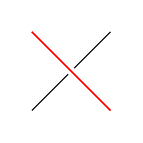
\begin{tikzpicture}[scale = 1]
                \draw (0,0) -- (1,1);
                \draw[draw=white,double=red,very thick] (0,1) -- (1,0);
            \end{tikzpicture}
        \end{minipage}
        \begin{minipage}{0.55\linewidth}
            \begin{lstlisting}[style = latex-side]
    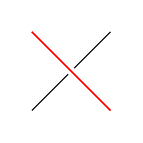
\begin{tikzpicture}[scale = 1]
        \draw (0,0) -- (1,1);
        \draw[draw=white,double=red,very thick] (0,1) -- (1,0);
    \end{tikzpicture}
            \end{lstlisting}
        \end{minipage}
        \caption{Path Style:double}
    \end{figure}

    \item double distance = <dimension> \hfill (默认:0.6pt)
    
    设置两条边线的距离。

    \begin{figure}[H]
        \centering
        \begin{minipage}{0.3\linewidth}
            \centering
            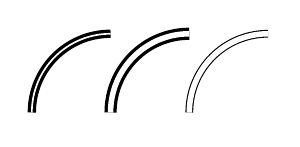
\begin{tikzpicture}[scale = 1]
                \draw[very thick,double] (0,0) arc (180:90:1cm);
                \draw[very thick,double distance=2pt] (1,0) arc (180:90:1cm);
                \draw[thin,double distance=2pt] (2,0) arc (180:90:1cm);
            \end{tikzpicture}
        \end{minipage}
        \begin{minipage}{0.6\linewidth}
            \begin{lstlisting}[style = latex-side]
    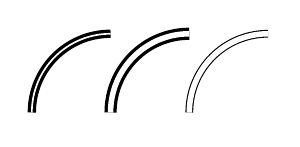
\begin{tikzpicture}[scale = 1]
        \draw[very thick,double] (0,0) arc (180:90:1cm);
        \draw[very thick,double distance=2pt] (1,0) arc (180:90:1cm);
        \draw[thin,double distance=2pt] (2,0) arc (180:90:1cm);
    \end{tikzpicture}
            \end{lstlisting}
        \end{minipage}
        \caption{Path Style:double distance}
    \end{figure}

    \item double distance between line centers = <dimension>
    
    该修饰与 double distance 类似,但它的距离计算是指两边线的中点的距离

    \begin{figure}[H]
        \centering
        \begin{minipage}{0.35\linewidth}
            \centering
            \begin{tikzpicture}[scale = 1]
                \begin{tikzpicture}
                    \foreach \lw in {0.5,1,1.5,2,2.5}
                        \draw[line width=\lw pt,double distance between line centers=3pt] (\lw,2em) -- ++(4mm,0);
                    \foreach \lw in {0.5,1,1.5,2,2.5}
                        \draw[line width=\lw pt,double distance = 3pt] (\lw,0) -- ++(4mm,0);
                \end{tikzpicture}
            \end{tikzpicture}
        \end{minipage}
        \begin{minipage}{0.55\linewidth}
            \begin{lstlisting}[style = latex-side]
    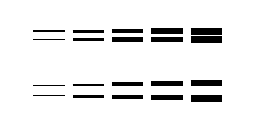
\begin{tikzpicture}
        \foreach \lw in {0.5,1,1.5,2,2.5}
            \draw[line width=\lw pt,double distance between line centers=3pt] (\lw,2em) -- ++(4mm,0);
        \foreach \lw in {0.5,1,1.5,2,2.5}
            \draw[line width=\lw pt,double distance = 3pt] (\lw,0) -- ++(4mm,0);
    \end{tikzpicture}
            \end{lstlisting}
        \end{minipage}
        \caption{Path Style:double distance between line centers}
    \end{figure}
\end{itemize}
    
\subsubsection{线条修饰}

启用 decorations.pathmorphing 包,可以启动多种线条样式。

\begin{figure}[H]
    \centering
    \begin{minipage}{0.35\linewidth}
        \centering
        \begin{tikzpicture}
            \node [circular drop shadow={shadow scale=1.05},minimum size=3.13cm,decorate, decoration=zigzag,fill=blue!20,draw,thick,circle] {Hello!};
        \end{tikzpicture}
    \end{minipage}
    \begin{minipage}{0.55\linewidth}
        \begin{lstlisting}[style = latex-side]
    \begin{tikzpicture}
        \node [circular drop shadow={shadow scale=1.05},minimum size=3.13cm,decorate, decoration=zigzag,fill=blue!20,draw,thick,circle] {Hello!};
    \end{tikzpicture}
        \end{lstlisting}
    \end{minipage}
    \caption{Path Style:decorate}
\end{figure}


\subsection{填充样式}

\subsubsection{填充图案}

TikZ 为我们提供了很多内置的图案用来填充,值得说明的是,这些图案并不能进行大小或方向的修改,除非我们重新定义一种图案。

\begin{itemize}
    \item pattern = <name>
    
    该修饰用来指定填充的图案。需要加载 patterns 包。
    \begin{figure}[H]
        \centering
        \begin{minipage}{0.35\linewidth}
            \centering
            \begin{tikzpicture}[scale = 1]
                \draw[pattern=dots] (0,0) circle (1cm);
                \draw[pattern=fivepointed stars] (0,0) rectangle (3,1);
            \end{tikzpicture}
        \end{minipage}
        \begin{minipage}{0.55\linewidth}
            \begin{lstlisting}[style = latex-side]
    \begin{tikzpicture}[scale = 1]
        \draw[pattern=dots] (0,0) circle (1cm);
        \draw[pattern=fivepointed stars] (0,0) rectangle (3,1);
    \end{tikzpicture}
            \end{lstlisting}
        \end{minipage}
        \caption{Path Style:pattern}
    \end{figure}

    这里简单给出几个图案样式值如下表:

    \begin{table}[H]
        \centering
        \caption{Path Style:patterns 部分样式}
        \label{table:Path Style:patterns 部分样式}
        \setlength{\tabcolsep}{4mm}
        \begin{tabular}{cc|cc}
            \toprule
            \textbf{样式名} & \textbf{样式} & \textbf{样式名} & \textbf{样式} \\
            \midrule
            horizontal lines & 横线 & vertical lines & 竖线 \\
            north east lines & 斜线 & north west lines & 斜线 \\
            grid & 网格 & crosshatch & 斜网格 \\
            dots & 点 & crosshatch dots & 点 \\
            fivepointed stars & 五角星 & sixpointed stars & 六芒星 \\
            bricks & 砖型 & checkerboard & 棋盘型 \\
            \bottomrule
        \end{tabular}
    \end{table}

    \item pattern color = <color>

    用于指定图案颜色

    \begin{figure}[H]
        \centering
        \begin{minipage}{0.35\linewidth}
            \centering
            \begin{tikzpicture}[scale = 1]
                \draw[pattern color=red,pattern=fivepointed stars] (0,0) circle (1cm);
                \draw[pattern color=blue,pattern=fivepointed stars] (0,0) rectangle (3,1);
            \end{tikzpicture}
        \end{minipage}
        \begin{minipage}{0.55\linewidth}
            \begin{lstlisting}[style = latex-side]
    \begin{tikzpicture}[scale = 1]
        \draw[pattern color=red,pattern=fivepointed stars] (0,0) circle (1cm);
        \draw[pattern color=blue,pattern=fivepointed stars] (0,0) rectangle (3,1);
    \end{tikzpicture}
            \end{lstlisting}
        \end{minipage}
        \caption{Path Style:pattern color}
    \end{figure}
\end{itemize}

\subsubsection{填充渐变}

\begin{itemize}
    \item shade 
    
    基本的渐变填充,默认产生一个从上到下的灰色渐变效果。
    \begin{figure}[H]
        \centering
        \begin{minipage}{0.35\linewidth}
            \centering
            
\begin{tikzpicture}[scale = 1]
                \shade (0,0) circle (1ex);
            \end{tikzpicture}
        \end{minipage}
        \begin{minipage}{0.55\linewidth}
            \begin{lstlisting}[style = latex-side]
    \shade (0,0) circle (1ex);
            \end{lstlisting}
        \end{minipage}
        \caption{Path Style:shade}
    \end{figure}

    \item shading = <name>
    
    比 shade 提供了过多的渐变样式,总体上由 axis,radial,ball 三种渐变样式。

    \begin{figure}[H]
        \centering
        \begin{minipage}{0.35\linewidth}
            \centering
            
\begin{tikzpicture}[scale = 1]
                \shadedraw [shading = axis] (0,0) rectangle (1,1);
                \shadedraw [shading = radial,xshift = 1.5cm] (0,0) rectangle (1,1);
                \shadedraw [shading = ball,xshift = 3cm] (0,0) rectangle (1,1);
            \end{tikzpicture}
        \end{minipage}
        \begin{minipage}{0.55\linewidth}
            \begin{lstlisting}[style = latex-side]
    \shadedraw [shading = axis] (0,0) rectangle (1,1);
    \shadedraw [shading = radial,xshift = 1.5cm] (0,0) rectangle (1,1);
    \shadedraw [shading = ball,xshift = 3cm] (0,0) rectangle (1,1);
            \end{lstlisting}
        \end{minipage}
        \caption{Path Style:shading}
    \end{figure}
\end{itemize}

我们最常用到的是线性渐变,下面姐扫两个线性渐变中常用到的修饰。

\begin{itemize}
    \item left/right color = <color>

    用来指定渐变色。
    \begin{figure}[H]
        \centering
        \begin{minipage}{0.35\linewidth}
            \centering
            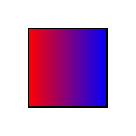
\begin{tikzpicture}[scale = 1]
                \shadedraw [left color=red,right color=blue] (0,0) rectangle (1,1);
            \end{tikzpicture}
        \end{minipage}
        \begin{minipage}{0.55\linewidth}
            \begin{lstlisting}[style = latex-side]
    \shadedraw [left color=red,right color=blue] (0,0) rectangle (1,1);
            \end{lstlisting}
        \end{minipage}
        \caption{Path Style:left/right color}
    \end{figure}

    \item shading angle = <degrees>
    
    可以用来改变线性渐变的角度。
    \begin{figure}[H]
        \centering
        \begin{minipage}{0.35\linewidth}
            \centering
            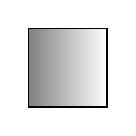
\begin{tikzpicture}[scale = 1]
                \shadedraw [shading=axis,shading angle=90] (0,0) rectangle (1,1);
            \end{tikzpicture}
        \end{minipage}
        \begin{minipage}{0.55\linewidth}
            \begin{lstlisting}[style = latex-side]
                \shadedraw [shading=axis,shading angle=90] (0,0) rectangle (1,1);
            \end{lstlisting}
        \end{minipage}
        \caption{Path Style:shading angle}
    \end{figure}
\end{itemize}

\subsection{路径范围}
\subsubsection{基础概念}

在讲述填充图案之前,我们需要了解 TikZ 的内部点计算方法。在默认情形下,我们总是对整个图案进行填充,但有时候我们需要对图案的交集等进行处理,这就需要了解到 TikZ 对内部点的判断两种算法。

\begin{itemize}
    \item nonzero rule
    
    TikZ 采用如下计算方式来计算是否为内部点:从某点出发沿任何方向绘制一条射线,如果射线遇到路径,采用以下方式计数:如果路径方向为从左到右,计数加一,如果路径方向为从右到左,计数减一。最终计数若非 0 则为内部点,否则为外部点。可形象地将外部视为中空区域。

    \begin{figure}[H]
        \centering
        \begin{minipage}{0.28\linewidth}
            \centering
            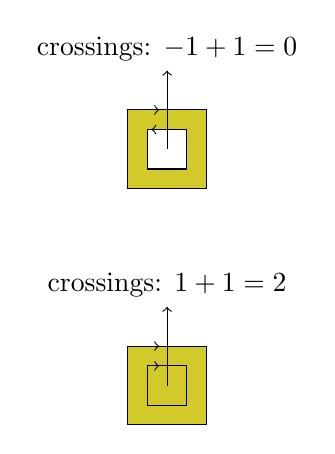
\begin{tikzpicture}
                \filldraw[fill=yellow!80!black]
                % Clockwise rectangle
                (0,0) -- (0,1) -- (1,1) -- (1,0) -- cycle
                % Counter-clockwise rectangle
                (0.25,0.25) -- (0.75,0.25) -- (0.75,0.75) -- (0.25,0.75) -- cycle;
                \draw[->] (0,1) -- (.4,1);
                \draw[->] (0.75,0.75) -- (0.3,.75);
                \draw[->] (0.5,0.5) -- +(0,1) node[above] {crossings: $-1+1 = 0$};
                \begin{scope}[yshift=-3cm]
                    \filldraw[fill=yellow!80!black]
                    % Clockwise rectangle
                    (0,0) -- (0,1) -- (1,1) -- (1,0) -- cycle
                    % Clockwise rectangle
                    (0.25,0.25) -- (0.25,0.75) -- (0.75,0.75) -- (0.75,0.25) -- cycle;
                    \draw[->] (0,1) -- (.4,1);
                    \draw[->] (0.25,0.75) -- (0.4,.75);
                    \draw[->] (0.5,0.5) -- +(0,1) node[above] {crossings: $1+1 = 2$};
                \end{scope}
            \end{tikzpicture}
        \end{minipage}
        \begin{minipage}{0.65\linewidth}
            \begin{lstlisting}[style = latex-side]
    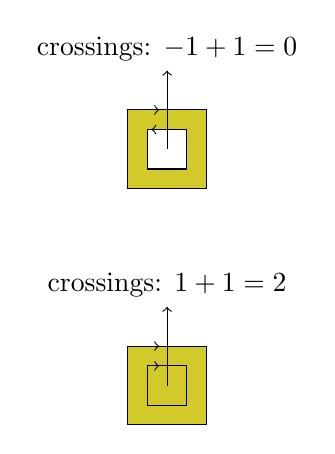
\begin{tikzpicture}
        \filldraw[fill=yellow!80!black]
        % Clockwise rectangle
        (0,0) -- (0,1) -- (1,1) -- (1,0) -- cycle
        % Counter-clockwise rectangle
        (0.25,0.25) -- (0.75,0.25) -- (0.75,0.75) -- (0.25,0.75) -- cycle;
        \draw[->] (0,1) -- (.4,1);
        \draw[->] (0.75,0.75) -- (0.3,.75);
        \draw[->] (0.5,0.5) -- +(0,1) node[above] {crossings: $-1+1 = 0$};
        \begin{scope}[yshift=-3cm]
            \filldraw[fill=yellow!80!black]
            % Clockwise rectangle
            (0,0) -- (0,1) -- (1,1) -- (1,0) -- cycle
            % Clockwise rectangle
            (0.25,0.25) -- (0.25,0.75) -- (0.75,0.75) -- (0.75,0.25) -- cycle;
            \draw[->] (0,1) -- (.4,1);
            \draw[->] (0.25,0.75) -- (0.4,.75);
            \draw[->] (0.5,0.5) -- +(0,1) node[above] {crossings: $1+1 = 2$};
        \end{scope}
    \end{tikzpicture}
            \end{lstlisting}
        \end{minipage}
        \caption{Path Style:nonzero rule}
    \end{figure}

    \item even odd rule
    
    另一种内部点算法:同样绘制射线,不进行减法运算,始终累计遇到的路径数,如果计算为奇数,则为内部点;否则为外部点。
    \begin{figure}[H]
        \centering
        \begin{minipage}{0.35\linewidth}
            \centering
            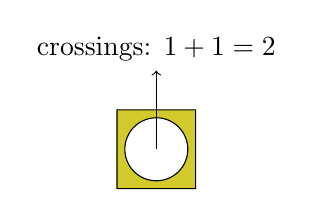
\begin{tikzpicture}
                \filldraw[fill=yellow!80!black,even odd rule]
                    (0,0) rectangle (1,1) (0.5,0.5) circle (0.4cm);
                \draw[->] (0.5,0.5) -- +(0,1) [above] node{crossings: $1+1 = 2$};
            \end{tikzpicture}
        \end{minipage}
        \begin{minipage}{0.55\linewidth}
            \begin{lstlisting}[style = latex-side]
    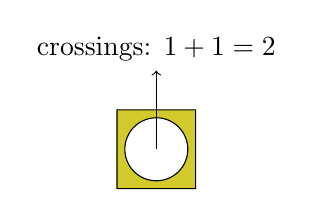
\begin{tikzpicture}
        \filldraw[fill=yellow!80!black,even odd rule]
            (0,0) rectangle (1,1) (0.5,0.5) circle (0.4cm);
        \draw[->] (0.5,0.5) -- +(0,1) [above] node{crossings: $1+1 = 2$};
    \end{tikzpicture}
            \end{lstlisting}
        \end{minipage}
        \caption{Path Style:even odd rule}
    \end{figure}

\end{itemize}

TikZ 还为我们提供了下面两个修饰对 path 路径创建的图形进行定位等操作。

\begin{itemize}
    \item path picture = <code>
    
    如果调用了修饰,那么在任何通过 \textbackslash path(及其衍生的 fill,shade 等)指令创建的图形,都会以此为基础创建一个 scope 区域,并在此区域中执行 <code>。

    \begin{figure}[H]
        \centering
        \begin{minipage}{0.35\linewidth}
            \centering
            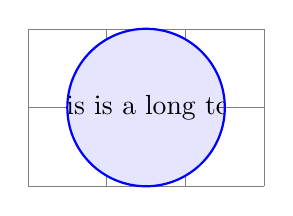
\begin{tikzpicture}
                \draw [help lines] (0,0) grid (3,2);
                \filldraw [fill=blue!10,draw=blue,thick] (1.5,1) circle (1)
                    [path picture={
                        \node at (path picture bounding box.center) {
                            This is a long text.
                        };}
                ];
            \end{tikzpicture}
        \end{minipage}
        \begin{minipage}{0.55\linewidth}
            \begin{lstlisting}[style = latex-side]
    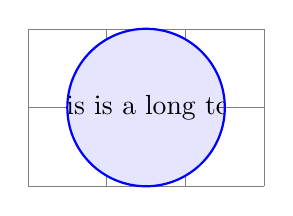
\begin{tikzpicture}
        \draw [help lines] (0,0) grid (3,2);
        \filldraw [fill=blue!10,draw=blue,thick] (1.5,1) circle (1)
            [path picture={
                \node at (path picture bounding box.center) {
                    This is a long text.
                };}
        ];
    \end{tikzpicture}
            \end{lstlisting}
        \end{minipage}
        \caption{Path Style:path picture}
    \end{figure}

    \item path picture bounding box
    
    任何创建的路径都可认为被包括在一个矩形框内,通过调用 path picture bounding box 可以获得矩形框的位置。

    \begin{figure}[H]
        \centering
        \begin{minipage}{0.35\linewidth}
            \centering
            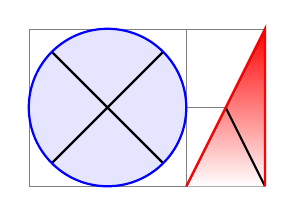
\begin{tikzpicture}[cross/.style={path picture={
                \draw[black]
                    (path picture bounding box.south east) --
                    (path picture bounding box.north west)
                    (path picture bounding box.south west) --
                    (path picture bounding box.north east);
                }}]
                \draw [help lines] (0,0) grid (3,2);
                \filldraw [cross,fill=blue!10,draw=blue,thick] (1,1) circle (1);
                \path [cross,top color=red,draw=red,thick] (2,0) -- (3,2) -- (3,0);
            \end{tikzpicture}
        \end{minipage}
        \begin{minipage}{0.55\linewidth}
            \begin{lstlisting}[style = latex-side]
    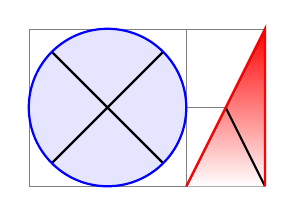
\begin{tikzpicture}[cross/.style={path picture={
        \draw[black]
            (path picture bounding box.south east) --
            (path picture bounding box.north west)
            (path picture bounding box.south west) --
            (path picture bounding box.north east);
        }}]
        \draw [help lines] (0,0) grid (3,2);
        \filldraw [cross,fill=blue!10,draw=blue,thick] (1,1) circle (1);
        \path [cross,top color=red,draw=red,thick] (2,0) -- (3,2) -- (3,0);
    \end{tikzpicture}
            \end{lstlisting}
        \end{minipage}
        \caption{Path Style:path picture bounding box}
    \end{figure}

\end{itemize}

\subsubsection{边界框}

在绘制图形的过程中,TikZ 会默认将所有点都包含在图片范围内,然而有时候我们会让某些点突破图片范围。

\begin{itemize}
    \item use as bounding box
    
    在某个路径中启用该修饰后,图像的边界框将由该路径确定,随后的路径不再对边界框有影响。然而如果之前的路径确定了更大的边界框,该修饰并不会使得边界框变小(可以通过 \textbackslash pgfresetboundingbox 重置边界框)。

    此外,该修饰因为常被用来指定边界框大小,TikZ 也提供了指令形式 \textbackslash useasboundingbox

    Left of picture
    
\begin{tikzpicture}
    \useasboundingbox (0,0) rectangle (3,1);
    \fill (.75,.25) circle (.5cm);
    \end{tikzpicture}
    right of picture.

    \begin{figure}[H]
        \centering
        \begin{minipage}{0.55\linewidth}
            \begin{lstlisting}[style = latex-side]
    Left of picture
        
\begin{tikzpicture}
            \useasboundingbox (0,0) rectangle (3,1);
            \fill (.75,.25) circle (.5cm);
        \end{tikzpicture}
    right of picture.
            \end{lstlisting}
        \end{minipage}
        \caption{Path Style:useasboundingbox}
    \end{figure}

    \item current bounding box
    
    边界框不仅可以被指定,也可以被调用:

    \begin{figure}[H]
        \centering
        \begin{minipage}{0.35\linewidth}
            \centering
            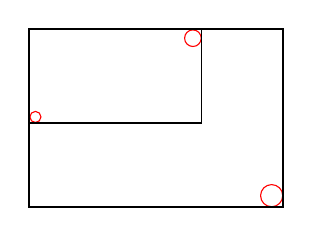
\begin{tikzpicture}
                \draw[red] (0,0) circle (2pt);
                \draw[red] (2,1) circle (3pt);
                \draw (current bounding box.south west) rectangle
                    (current bounding box.north east);
                \draw[red] (3,-1) circle (4pt);
                \draw[thick] (current bounding box.south west) rectangle
                    (current bounding box.north east);
            \end{tikzpicture}
        \end{minipage}
        \begin{minipage}{0.55\linewidth}
            \begin{lstlisting}[style = latex-side]
    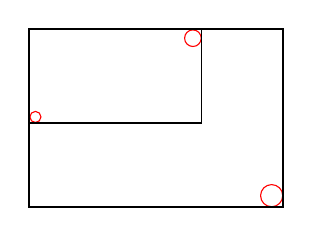
\begin{tikzpicture}
        \draw[red] (0,0) circle (2pt);
        \draw[red] (2,1) circle (3pt);
        \draw (current bounding box.south west) rectangle
            (current bounding box.north east);
        \draw[red] (3,-1) circle (4pt);
        \draw[thick] (current bounding box.south west) rectangle
            (current bounding box.north east);
    \end{tikzpicture}
            \end{lstlisting}
        \end{minipage}
        \caption{Path Style:current bounding box}
    \end{figure}

    \item trim left = <dimension or coordinate>  \hfill (默认:0pt)
    
    该修饰将传入的值设置为边界框的左边界,如果是坐标,则只使用 x 值。

    Text before image.%
    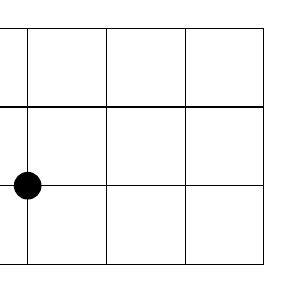
\begin{tikzpicture}[trim left]
    \draw (-1,-1) grid (3,2);
    \fill (0,0) circle (5pt);
    \end{tikzpicture}%
    Text after image.

    \begin{figure}[H]
        \centering
        \begin{minipage}{0.55\linewidth}
            \begin{lstlisting}[style = latex-side]
    Text before image.%
    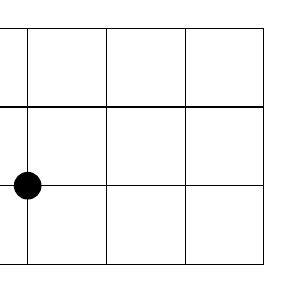
\begin{tikzpicture}[trim left]
    \draw (-1,-1) grid (3,2);
    \fill (0,0) circle (5pt);
    \end{tikzpicture}%
    Text after image.
            \end{lstlisting}
        \end{minipage}
        \caption{Path Style:useasboundingbox}
    \end{figure}

    \item trim right = <dimension or coordinate>
 
\end{itemize}

\subsubsection{剪裁蒙版}

剪裁路径是指将绘制的路径限定在一定的区域内,作用类似于 PS 的蒙版遮罩。

\begin{itemize}
    \item clip
    
    该修饰对应的路径将作为蒙版,在整个 scope 中起作用。

    \begin{figure}[H]
        \centering
        \begin{minipage}{0.35\linewidth}
            \centering
            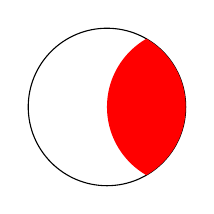
\begin{tikzpicture}[scale = 1]
                \draw[clip] (0,0) circle (1cm);
                \fill[red] (1,0) circle (1cm);
            \end{tikzpicture}
        \end{minipage}
        \begin{minipage}{0.55\linewidth}
            \begin{lstlisting}[style = latex-side]
    \begin{tikzpicture}[scale = 1]
        \draw[clip] (0,0) circle (1cm);
        \fill[red] (1,0) circle (1cm);
    \end{tikzpicture}
            \end{lstlisting}
        \end{minipage}
        \caption{Path Style:clip}
    \end{figure}

    TikZ 提供了指令形式的 \textbackslash clip。

    \begin{figure}[H]
        \centering
        \begin{minipage}{0.35\linewidth}
            \centering
            \begin{tikzpicture}[scale = 2]
                \draw (0,0) -- ( 0:1cm);
                \draw (0,0) -- (10:1cm);
                \draw (0,0) -- (20:1cm);
                \draw (0,0) -- (30:1cm);
                \begin{scope}[fill=red]
                    \clip[fill] (0.2,0.2) rectangle (0.5,0.5);
                    \draw (0,0) -- (40:1cm);
                    \draw (0,0) -- (50:1cm);
                    \draw (0,0) -- (60:1cm);
                \end{scope}
                \draw (0,0) -- (70:1cm);
                \draw (0,0) -- (80:1cm);
                \draw (0,0) -- (90:1cm);
            \end{tikzpicture}
        \end{minipage}
        \begin{minipage}{0.55\linewidth}
            \begin{lstlisting}[style = latex-side]
    \begin{tikzpicture}[scale = 2]
        \draw (0,0) -- ( 0:1cm);
        \draw (0,0) -- (10:1cm);
        \draw (0,0) -- (20:1cm);
        \draw (0,0) -- (30:1cm);
        \begin{scope}[fill=red]
            \clip[fill] (0.2,0.2) rectangle (0.5,0.5);
            \draw (0,0) -- (40:1cm);
            \draw (0,0) -- (50:1cm);
            \draw (0,0) -- (60:1cm);
        \end{scope}
        \draw (0,0) -- (70:1cm);
        \draw (0,0) -- (80:1cm);
        \draw (0,0) -- (90:1cm);
    \end{tikzpicture}
            \end{lstlisting}
        \end{minipage}
        \caption{Path Style:\textbackslash clip}
    \end{figure}
\end{itemize}

\subsection{复杂动作}

通常 TikZ 绘制路径的顺序为: fill - draw - clip。然而有的时候我们需要对路径进行更为复杂的操作,例如多次填充图案等。

\begin{itemize}
    \item preaction = <options>
    
    当给 path 该修饰时,会创建一个对应的 scope。在这个 scope 中会首先强制执行 <options> 中的修饰,再执行其他修饰。

    \begin{figure}[H]
        \centering
        \begin{minipage}{0.35\linewidth}
            \centering
            \begin{tikzpicture}[scale = 1]
                \draw[help lines] (0,0) grid (3,2);
                \draw [preaction={draw,line width=4mm,blue}]
                    [line width=2mm,red] (0,0) rectangle (2,2);
            \end{tikzpicture}
        \end{minipage}
        \begin{minipage}{0.55\linewidth}
            \begin{lstlisting}[style = latex-side]
    \begin{tikzpicture}[scale = 1]
        \draw[help lines] (0,0) grid (3,2);
        \draw [preaction={draw,line width=4mm,blue}]
            [line width=2mm,red] (0,0) rectangle (2,2);
    \end{tikzpicture}
            \end{lstlisting}
        \end{minipage}
        \caption{Path Style:preaction}
    \end{figure}

    同一个 path 可以拥有多个 preaction,以达到在同一个路径上多次绘制的效果。
    
    \begin{figure}[H]
        \centering
        \begin{minipage}{0.35\linewidth}
            \centering
            \begin{tikzpicture}
                \draw[help lines] (0,0) grid (3,2);
                \draw [pattern=fivepointed stars]
                    [preaction={fill=black,opacity=.5, transform canvas={xshift=1mm,yshift=-1mm}}]
                    [preaction={top color=blue,bottom color=white}]
                        (0,0) rectangle (1,2)
                        (1,2) circle (5mm);
            \end{tikzpicture}
        \end{minipage}
        \begin{minipage}{0.55\linewidth}
            \begin{lstlisting}[style = latex-side]
    \begin{tikzpicture}
        \draw[help lines] (0,0) grid (3,2);
        \draw [pattern=fivepointed stars]
            [preaction={fill=black,opacity=.5, transform canvas={xshift=1mm,yshift=-1mm}}]
            [preaction={top color=blue,bottom color=white}]
                (0,0) rectangle (1,2)
                (1,2) circle (5mm);
    \end{tikzpicture}
            \end{lstlisting}
        \end{minipage}
        \caption{Path Style:multi-preaction}
    \end{figure}

    \item postaction = <options>
    
    postaction 与 preaction 类似,只不过再其他修饰执行后再执行 postaction 中的修饰。

    \begin{figure}[H]
        \centering
        \begin{minipage}{0.35\linewidth}
            \centering
            \begin{tikzpicture}
                \draw[help lines] (0,0) grid (3,2);
                \draw
                    [postaction={draw,line width=2mm,blue}]
                    [line width=4mm,red,fill=white] (0,0) rectangle (2,2);
            \end{tikzpicture}
        \end{minipage}
        \begin{minipage}{0.55\linewidth}
            \begin{lstlisting}[style = latex-side]
    \begin{tikzpicture}
        \draw[help lines] (0,0) grid (3,2);
        \draw
            [postaction={draw,line width=2mm,blue}]
            [line width=4mm,red,fill=white] (0,0) rectangle (2,2);
    \end{tikzpicture}
            \end{lstlisting}
        \end{minipage}
        \caption{Path Style:postaction}
    \end{figure}

\end{itemize}

\newpage